\documentclass[11pt,a4paper,twoside]{report}
    \usepackage{a4wide}
    \usepackage{epsfig}
    \usepackage{amsmath}
    \usepackage{tabu}
    \usepackage{amsfonts}
    \usepackage{latexsym}
    \usepackage[utf8]{inputenc}
    \usepackage{listings}
    \usepackage{color}
    \usepackage{titlesec}    
    \usepackage{enumitem}
    \usepackage[catalan]{babel}
    \usepackage{newunicodechar}
    \usepackage{graphicx}
    \usepackage{subcaption}
    \usepackage{float}
    \usepackage{xcolor}
    \usepackage{pgf, tikz}
    \usepackage{listings}
    \usepackage{booktabs}
    \usepackage[sorting=none]{biblatex}
    \usepackage{eurosym}
    \usepackage[figuresleft]{rotating}
    \usepackage{mathtools}

    \addbibresource{bibliography.bib}
    \bibliography{bibliography}
    
  \setcounter{tocdepth}{4}
  \setcounter{secnumdepth}{4}
  
  \newunicodechar{Ŀ}{\L.}
  \newunicodechar{ŀ}{\l.}
  \definecolor{dkgreen}{rgb}{0,0.6,0}
  \definecolor{gray}{rgb}{0.5,0.5,0.5}
  \definecolor{mauve}{rgb}{0.58,0,0.82}
  
  \DeclareSourcemap{
  \maps[datatype=bibtex]{
    \map{
      \step[fieldsource=howpublished, match=\regexp{\A\\url\{(.+ | $)\}\Z}, final]
      \step[fieldset=url, fieldvalue={$1}]
      \step[fieldset=howpublished, null]
    }
  }
}
\definecolor{maroon}{rgb}{0.5,0,0}
\definecolor{darkgreen}{rgb}{0,0.5,0}
\lstdefinelanguage{XML}
{
  basicstyle=\ttfamily,
  morestring=[s]{"}{"},
  morecomment=[s]{?}{?},
  morecomment=[s]{!--}{--},
  commentstyle=\color{darkgreen},
  moredelim=[s][\color{black}]{>}{<},
  moredelim=[s][\color{red}]{\ }{=},
  stringstyle=\color{blue},
  identifierstyle=\color{maroon}
}

  \usepackage{hyperref}
  \hypersetup{
    colorlinks=false, %set true if you want colored links
    linktoc=all,     %set to all if you want both sections and subsections linked
    linkcolor=blue,  %choose some color if you want links to stand out
  }
  
  \setlength{\footskip}{50pt}
  \setlength{\parindent}{0cm} \setlength{\oddsidemargin}{-0.5cm} \setlength{\evensidemargin}{-0.5cm}
  \setlength{\textwidth}{17cm} \setlength{\textheight}{23cm} \setlength{\topmargin}{-1.5cm} \addtolength{\parskip}{2ex}
  \setlength{\headsep}{1.5cm}
  
  \renewcommand{\contentsname}{Continguts}
  \setcounter{chapter}{0}
  % \titleformat{\chapter}[display]
  % {\normalfont\bfseries}{}{0pt}{\Large}
  \titleformat{\chapter}[block]
  {\normalfont\LARGE\bfseries}{\thechapter.}{1em}{\LARGE}
  \titleformat{\section}[block]
  {\normalfont\Large\bfseries}{\thesection.}{1em}{\Large}
  
  \begin{document}
  \tableofcontents
  
  \chapter{Introducció, motivacions, propòsit i objectius}
  
  % \section{Introducció}
  % \section{Motivacions}
  % \section{Propòsit}
  % \section{Objectius}

  La confecció d'horaris és un problema recorrent amb el que es troben els instituts que amaga una alta combinatòria, dificultant-ne molt la seva elaboració manual posat que s'han de prendre moltíssimes decisions a cegues,
  fent que sigui molt probable cometre errors en la confecció. En aquesta situació, amb la aparició dels computadors molts instituts varen decidir ajudar-se en aquesta tasca utilitzant eines informàtiques capaces 
  d'explorar grans quantitats de combinacions per segon. No obstant a això, amb aquelles primeres eines es seguien tenint molts problemes per generar horaris viables, que normalment eren de qualitat baixa 
  i requerien un refinament posterior que s'havia de fer de forma manual.
  
  El HSTT (High School TimeTabling) consisteix en la solució de forma automàtica de aquest problema d'alta complexitat (NP). 
  Així doncs, el que s'intenta és la configuració automàtica de horaris de institut partint de una sèrie de recursos 
  (per exemple: aules, professors, assignatures, grups) i repartir-los de manera que sigui viable i tenint en compte 
  de manera total o parcial les preferències del professorat en quant a horaris, continuïtat, grups, etc. Tot aixó fa que el problema sigui molt difícil de resoldre, degut al gran nombre de combinacions possibles entre els diferents recursos.
  
  Afegint dificultat al problema, depenguen del país del qual estiguem parlant existeixen una gran diversitat de requisits propis, degut a les característiques pròpies del sistema d'estudis secundaris de cada lloc.

  Degut a tot el mencionat encara no existeix cap eina capaç de trobar una solució òptima al problema de manera determinista en un temps raonable, encara que s'ha avançat molt en la resolució de problemes d'aquest tipus i costen de trobar instituts que optin per fer els horaris de forma manual.
  
  Els objectius d'aquest treball són els següents:
  \begin{itemize}
    \item Aprofundir sobre el problema de la generació d'horaris en sí i sobre els problemes de satisfacció de restriccions en general i les tècniques que s'utilitzen per resoldre'ls, com ara, SAT i les seves diverses extensions.
    \item Desenvolupar un generador d'horaris automàtic utilitzant les tècniques estudiades anteriorment, aprofitant les eines relacionades que s'han desenvolupades recentment pel grup de recerca Lògica i Programació, que resolgui el problema en un temps raonable i intenti trobi la millor solució possible, 
    cosa que es preveu molt complicada d'aconseguir en un temps raonable en les instàncies grosses.
    
  \end{itemize}
  
  \section{Grup de recerca Lògica i Programació}
  Aquest treball s'emmarca dins del grup de recerca de Lògica i Programació de l'àmbit d'àrea tècnica de la Universitat de Girona.

  El grup basa la seva recerca en l'estudi de satisfactibilitat de formules proposicionals booleanes (SAT) i Satisfiability Modulo Theories (SMT) i les seves
  aplicació per a la resolució de problemes combinatoris com ara problemes de \textit{scheduling} i \textit{planning} arribant a utilitzar amb èxit tècniques innovadores en altres àmbits com
  pot ser: els problemes de \textit{scheduling} i \textit{planning}.

  Durant la elaboració del treball he rebut ajuda i assessorament dels membres del grup, incloent el meu tutor de projecte, el Dr. Josep Suy, qui també en forma part.

  \section{Estructura del Treball}
  A continuació s'exposa l'estructura d'aquest document: 
  \begin{enumerate}
    \item Introducció, motivacions, propòsit i objectius: Situa el marc del projecte, explica les raons per les quals s'ha escollit el treball i en defineix els objectius.
    \item Estudi de viabilitat: Justifica la capacitat de fer el projecte
    \item Metodologia i Planificació: Tot i que a la guía van separats, s'ha decidit ajuntar-los per la gran relació que tenen entre ells. En aquest apartat s'exposa la metodologia que s'ha seguit a la hora de implementar el projecte i es defineix l'estratègia seguida per arribar als objectius.
    \item Marc de treball i conceptes prèvis: S'exposa el treball prèvi realitzat sobre el problema, i els coneixements necessaris per a la implementació del programa.
    \item Requisits del sistema: Requisits funcionals i no funcionals que ha de complir el sistema.
    \item Anàlisi i disseny del sistema: Descripció del maquinari i programari utilitzat durant el desenvolupament del projecte.
    \item Implementació i proves: Es detalla la implementació del programa, els problemes que han aparegut i les solucions que s'han donat a aquests.
    \item Implantació i resultats: Detalla els resultats obtinguts.
    \item Conclusions: Conclusió del projecte i els resultats
    \item Treball futur: Possibles ampliacions, millores o treballs futurs que es poden realitzar.
    \item Bibliografía: Referències utilitzades per desenvolupar el projecte.
    \item Manual d'usuari i insta\l.lació: Especifica les passes a seguir per utilitzar el sistema creat en un ordinador.

  \end{enumerate}

%   La introducció serveix per situar el marc del projecte. Aquesta primera etapa implica
% establir les raons que justificaven el desenvolupament del projecte i el que se
% n’esperava obtenir. Aquest propòsit és, per naturalesa, una idea molt ampla.
% Pel contrari, els objectius identifiquen les fites específiques que l’estudiant esperava
% assolir en el seu camí cap al propòsit últim del projecte. Els objectius són més
% precisos que el propòsit general. A partir d’aquesta informació s’ha de comprendre
% millor el projecte, identificar l’entorn on es desenvolupa i entendre millor quina és la
% feina que ha calgut fer.
% En l’apartat anterior, cal precisar i no confondre entre el que són els objectius del
% projecte i els requisits del producte final (aplicació, sistema de maquinari,
% algorismes...).
% En cas que el projecte es desenvolupi en un entorn consolidat (grup de recerca,
% empresa, institució...), aquest apartat pot incloure una descripció de l’entorn en el
% qual es desenvolupa el projecte, així com una especificació del punt de partida del
% projecte. També cal deixar clar en aquest punt quina és l’aportació del P/TFC en
% relació amb el punt de partida.
% En aquest apartat l’estudiant també ha de justificar els apartats de la memòria
% afegits, suprimits o canviats d’ordre respecte del que descriu aquest document.
  \chapter{Estudi de viabilitat}

  \section{Viabilitat tècnica}

  Per tal de realitzar aquest projecte farà el software necessari per poder tractar un fitxer XML, codificar una instància del problema en C++ i resoldre-la amb un \textit{solver} SAT o d'alguna extensió de SAT. 
  Abans de iniciar el projecte, s'ha comprovat l'existència d'aquest software i que aquest estigués disponible de forma gratuïta, de fet, tot el software que s'utilitzi en aquest projecte serà de codi obert.

  Per part dels requisits de maquinari, tot i que HSTT és un problema dur, 
  després de veure el treball previ realitzat en aquest mateix problema i d'altres de característiques semblants, s'ha determinat que la meva màquina d'ús diari és més que suficient per a tal de realitzar el desenvolupament del generador d'horaris.

  Pel que fa a la habilitat de desenvolupar aquest treball s'ha determinat que era possible degut a que 
  el grup de recerca Lògica i Programació ha treballat i aconseguit solucionar problemes semblants de forma exitosa utilitzant tècniques innovadores. 
  Utilitzant els avenços fets pel grup s'ha decidit que es podria desenvolupar el treball en el marc de temps desitjat.



  \section{Viabilitat econòmica}
  
  Degut a que tot el software utilitzat és gratuït, lliure i de codi obert, i que el codi que el grup de recerca m'ha cedit també ha estat gratuït. Per part del maquinari, només s'ha utilitzat el que ja tenia amb anterioritat, així que per aquesta banda tampoc ha suposat cap cost.
  Així doncs, aquest projecte no s'ha requerit de cap inversió ni despesa econòmica. 
  Així doncs l'únic cost que ha suposat aquest treball han estat el temps necessari per fer-lo i les ganes que se li han hagut de ficar. 


  \subsection{Pressupost}
  Tot i que, com s'ha explicat anteriorment, el desenvolupament d'aquest treball no té cost, s'ha decidit fer una simulació del que costaria contractar un programador per fer el treball.
  
  \begin{center}
    \begin{tabular}{|| c | c | c | c||} 
    \hline
     & \euro/h & Hores & Cost \\ [0.5ex] 
    \hline\hline
    Programador & 14 & 180 & 2520 \\ [1ex] 
    \hline
   \end{tabular}
   \end{center}

   A part també s'han de tenir en compte el maquinari utilitzat:
   \begin{center}
    \begin{tabular}{|| c | c | c | c||} 
    \hline
     & Cost Total & Hores & \euro/h \\ [0.5ex] 
    \hline\hline
    Ordinador Principal & 828 & 170 & 4.9 \\ [1ex] 
    Ordinador Portatil Secundari & 200 & 10 & 20 \\ [1ex] 
    \hline\hline
    Total & 1028 & 190 & 5.71 \\


    \hline
   \end{tabular}
   \end{center}


   També cal tenir en compte que els tutors del treball m'han ajudat molt, i han dedicat part del seu temps en les reunions, intercanvis de mails i conversacions que s'han tingut sobre el treball.
   \begin{center}
    \begin{tabular}{|| c | c ||} 
    \hline
     & Hores \\ [0.5ex] 
    \hline\hline
    Josep Suy & 20 \\ [1ex] 
    Jordi Coll & 10 \\ [1ex] 
    \hline
   \end{tabular}
   \end{center}
  % preguntar suy
  %==================
  % Cal justificar quins són els paràmetres que feien possible el desenvolupament del
  % projecte. Aquest punt pot incloure els recursos necessaris per desenvolupar el
  % projecte, els pressupostos inicials, la viabilitat tecnològica i/o econòmica, els
  % recursos humans, etc.
  %

  \chapter{Metodologia i Planificació}
  \section{Metodologia}
  La part més important i grossa d'aquest treball és la creació d'un generador automàtic d'horaris utilitzant les eines oferides per el grup de recerca. 
  Primer caldrà estudiar el problema (HSTT) i la seva duresa, per poder ser capaç d'entendre el què estem treballant.
  Des de aquí es procedirà a la implementació del programa, utilitzant la API SMT creada per el Dr. Jordi Coll, el qual es membre del grup de recerca de Lògica i Programació del departament de Informàtica, Matemàtica Aplicada i Estadística.
  Aquesta API ens estalviarà la codificació de les restriccions de cardinalitat i les restriccions pseudo-booleanes, 
  apart de oferir-nos una interfície senzilla per poder implementar el model en diferents encodings i múltiples opcions.

  Després de fer un estudi preliminar del problema i el treball prèvi respecte aquest, la metodologia de treball que s'ha seguit ha estat la de entregues periòdiques. 
  Consistint en fer una reunió amb els tutors per decidir el pròxim pas del treball i jo dedicar-me durant un temps a fer aquest pas. Després d'aquest temps es convoca una altre reunió on es valora el treball fet i es decideix com seguir. 
  Des de aquí es va repetint fins a acabar el projecte.

  %1 - estudiar el problema
  %2 - fer el parser
  %3 - testejar el parser
  %4 - estudi yices
  %5 - estudi api smt jordi coll
  %6 - fer model
  %7 - testing model
  %8 - proves diferents encodings de les cardinality constraints
  %9 - millora format output
  %10 - si cal, confeccio model
  \section{Planificació}

  Com s'ha dit en l'apartat anterior primer caldrà estudiar el problema HSTT i la seva duresa. 
  Després es procedirà amb el disseny i la implementació del generador. Primer caldrà dissenyar implementar i testejar un \textit{parser} pels fitxers. En aquest pas també cal pensar i implementar en quina estructura es guardaràn aquestes dades i com es transferiràn en el model que es codificarà posteriorment. 

  Al tenir el \textit{parser} i l'estructura de dades enllestits caldrà començar a estudiar com funciona la API per C++ del Yices i 
  posteriorment la API SMT del Dr. Jordi Coll. Això ens permetrà començar a dissenyar, codificar i testejar el model, que és el següent pas del treball. 
  Al tenir enllestit el model, es faràn les proves de rendiment amb diferents límits de optimització i diferents encodings de les restriccions de cardinalitat.
  Finalment s'implementarà una forma maca i llegible de mostrar els horaris generats.
  
  Amb això el generador es donarà per acabat i es passarà a la confecció de la memòria del treball. 
  A continuació un diagrama de Gantt mostrant la planificació feta.

  %% diagrama de gantt...

  %% CAL AMPLIAR

  \begin{figure}
    \centering
    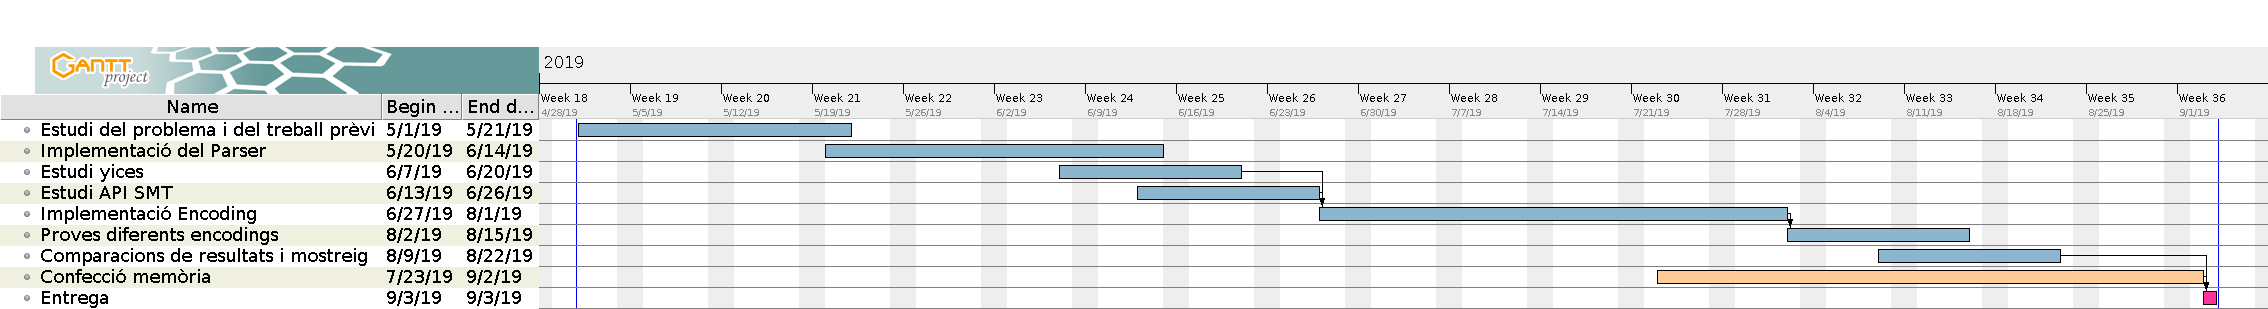
\includegraphics[angle=90,origin=c,height=0.58\textheight]{Diagrames/gantt1.png} 
    \caption{Diagrama de Gantt}
    \label{fig:Gantt}
  \end{figure}




  \chapter{Marc de treball i conceptes prèvis}
  \section{Marc de treball}
    Com s'ha mencionat en la introducció aquest treball s'emmarca dins del grup de recerca de Lògica i Programació (LAP) del departament de Informàtica, Matemàtica Aplicada i Estadística (IMAE) de la Universitat de Girona. 
    En el treball s'utilitzaràn les eines desenvolupades recentment en el grup de recerca, per ser exactes, la API SMT feta en C++ per el Dr. Jordi Coll. 
    Aquesta API permet codificar problemes SAT, MaxSAT i SMT per a diferents solvers de forma transparent a aquest i te implementades les diferents restriccions de cardinalitat i pseudo-booleanes en les diferents possibles codificacions. 
    També inclou diferents algoritmes d'optimització implementats.

    La resta del treball prévi seria el treball també sobre confecció d'horaris d'institut fet el 2015 per en Cristòfor Nogueira\cite{treballCristo}
    %nose seguir  
    %s'ha de mencionar el treball den cristofol, probablament, 

  \section{Definició del problema}
    El problema que es treballa és el de la confecció d'horaris per a institut (HSTT de \textit{High School Time Tables}). 
    Aquest consisteix en assignar a cada assignatura que es fa en un centre l'espai de temps en que s'impartirà i el conjunt de recursos que utilitzarà. 
    Els recursos normalment seràn professors i aules, però es contemplen altres possibles necessitats especials de cada centre, per això es generalitza.

    La duresa de aquest problema es troba en assignar un espai de temps per a cada assignatura donant-li els recursos que necessita sense violar cap restricció que aquests tinguin, 
    com podria ser no fer dues assignatures a la vegada en la mateixa aula, o sigui, que al realitzar-se la assignatura tots els seus recursos estiguin disponibles.  
    De la mateixa manera es poden imposar diverses restriccions de naturaleses diferents i amb cada una s'aniràn reduint les possibles combinacions vàlides i fent més i més difícil la generació del horari.
    \subsection{Estudi de duresa}

    

    \subsubsection{Incís en la teoría de la computació}
    Abans de procedir a l'estudi de la duresa del problema HSTT, caldrà explicar els següents conceptes de la teoria de la computació: 
    \paragraph*{Problemes decidibles i indecidibles}

    Un problema decidible és aquell per el qual existeix una màquina de Turing que para en totes les entrades possibles amb una resposta: sí o no. Aquests problemes també són coneguts com a Turing Decidibles. 
    Així doncs, un problema decidible és aquell pel qual sempre podrem construir un algorisme que sempre respon el problema.
    
    Un problema pot ser semi-decidible, això passa quan una màquina de turing quan l'entrada és acceptada, però es pot penjar o es pot parar quan l'entrada es rebutja. Aquests problemes també son referits com a Turing Reconeixibles.
    
    Un problema indecidible és aquell pel qual no podem construir un algorisme que resolgui el problema en temps finit. Aquests problemes poden ser parcialment decidibles, però sempre hi haurà una condició que portara la màquina de Turing a bucle infinit.


    \paragraph*{P, NP i NP-Completesa}
    \begin{itemize}
      \item \textbf{P: }És el conjunt de problems que poden ser resolts en temps polinòmic amb una màquina de Turing determinista. 
      \item \textbf{NP: }És el conjunt de problemes que poden ser resolts en temps polinòmic amb una màquina de Turing no determinista. 
      \item \textbf{NP-Complet: }És el conjunt de problemes més durs en el conjunt NP. Un problema C és NP-Complet si C és NP i tot problema NP és reduïble a C.
      \item \textbf{NP-Hard: }És el conjunt de problemes als quals es pot reduïr tot problema NP. O sigui, un problema C és NP-Hard si tot problema NP és reduïble a C. 
      \item \textbf{Reducció: }Si tenim dos problemes $L_1$ i $L_2$  i tenim un algoritme $A_2$ que resol $L_2$. Reduir $L_1$ a $L_2$ és transformar el problema $L_1$ a $L_2$ així poder utilitzar el algoritme $A_2$ per resoldre el problema, creant així un algoritme $A_1$ amb l'estructura que es pot veure en la figura \ref{fig:reduccio}
      \begin{figure}[ht!]
        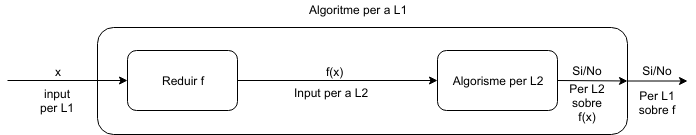
\includegraphics[width=\textwidth]{Diagrames/Reduccio.png}
        \caption{Esquema de Reducció}
        \label{fig:reduccio}
      \end{figure}
      
    \end{itemize}

    \subsubsection{Duresa de HSTT}
    El problema HSTT és clarament decidible i, posat que comprovar si una solució satisfà totes les restriccions imposades és d'ordre polinòmic, aquest pertany al conjunt de problemes NP.
    
    \paragraph*{NP-Completesa de HSTT} ~\\

    En aquest apartat s'inclou la demostració que es veu en el treball d'en Cristòfor Nogueira\cite{treballCristo}.
    
    Es pot demostrar la NP-Completesa del problema HSTT reduint un problema NP-Complet conegut a HSTT, en aquest cas, el problema de la motxilla\cite{wiki:bin}, d'acord amb la demostració proposada per B. Cooper i J.H. Kingston \cite{complexityHSTT}.

    Una de les fonts de la duresa del problema ve a l'hora de gestionar els recursos de manera coherent. Així que al confeccionar un horari serà d'interès mantenir el nombre d'incoherències per sota un llindar. 
    Les instànces HSTT acostumen a tenir com a mínim un tipus de recurs que compleix aquestes premises. 
    En cas q no en tinguin, és possible realitzar una transformació binària per arribar a aquesta formulació, 
    ja que tots els recursos poden atendre a un nombre limitat d'assignatures de manera simultània i totes les instàncies disposen d'un nombre limitat de recursos. Per tant, i per simplificar, considerarem només un únic recurs, de disponibilitat limitada. També considerarem que un recurs només pot atendre a una assignatura alhora.

    Diem que dues assignatures són incoherents si comparteixen algun espai de temps. És a dir, si es solapen. Com que els recursos són limitats interessa limitar el nombre de solapaments. Utilitzarem una codificació del problema de la motxilla per representar aquesta situació.

    El problema de la motxilla consisteix en determinar si un conjunt d'ítems $U = \{u_1, u_2, ..., u_n\}$, cadascun amb un pes associat $w_i$, es poden co\l.locar en un conjunt de motxilles $B = \{b_1, b_2, ..., b_m\}$, 
    cadascuna amb una capacitat màxima $c_i$ de manera que cap motxilla sobreexcedeixi la seva capacitat.

    Transformem el problema de la motxilla al següent problema HSTT: 
    \[
        Times = \{t_1,1, ..., t_n,m\}
    \]\[
        Events = X \cup Y, X = \{x_1, ..., x_n\} Y = \{y_1, ..., y_m\}
    \]

    De manera que: 
    \begin{itemize}
      \item A cada $x_i$ se li han d'assignar tants espais de temps com $w_i$.
      \item A cada $y_i$ se li han d'assignar tants espais de temps com $c_i$ i els corresponents a la motxilla que representen. És a dir, $y_i$ tindrà assignats els espais de temps $\{t_i,1 ... t_{i,c_i}\}$
    \end{itemize}
    
    El problema doncs, rau en determinar quins espais de temps s'assignen a cada $x_i$. 
    Suposem que aquest problema formulat com el de la motxilla té solució: $f: U \rightarrow B$ on el valor de retorn de $f$ és l'index de la motxilla on s'ha de co\l.locat l'ítem d'entrada. 
    Llavors, per cada assignatura $x_i$, escollim $w_i$ espais de temps, q no hagin estat escollits prèviament, del conjunt $S_k = \{t_k,1 ... t_{k, c_k}\}$, on $k = f(u_i)$. 
    Es a dir, s'escullen tants espais de temps com el pes de l'ítem que representa de manera que no hi hagin solapaments entre els membres de X. Aquest procés és possible perquè $f$ ens garanteix que com a molt s'escolliran $c_k$ espais de temps de $S_k$. 
    Al final tenim que tots els events tenen assignats exactament $w_i$ espais de temps i cada $X_i$ se solapa amb un, i només un event de $Y$. Per tant, tenim que el nombre d'incoherències o solapaments és $n$.
    
    Ara, suposem que la instància que la instància HSTT que hem descrit genera una solució amb un nombre de solapaments $\leq n$. Sabem que com a mínim el nombre de solapaments ha de ser $\geq n$, ja que cada $x_i$ 
    s'ha de solapar com a mínim una vegada amb algun membre de Y. Per tant el nombre de solapaments de la solució generada per la instància HSTT ha de ser exactament n i cada event $x_i$ es solapa només una vegada amb un sol membre de $Y$.
    Podríem reimplementar, doncs, $f$ de manera que a partir de la solució obtinguda per la instància HSTT es limiti a esbrinar per cada event $u_i$, amb quint event $y_i$ es solapa, de manera que $f(u_i) =j$.

  \section{Format XHSTT}
  Un dels problemes que presenta HSTT és la complexitat que té representar una instància amb totes les possibles restriccions possibles. Per això s'ha optat utilitzar el format genèric de instanciació de HSTT anomenat XHSTT (de \textit{Xml-format High School TimeTabling}) utilitzat per HSEval\cite{xhstt}.
  Aquest format és obert i preveu l'addició d'elements i restriccions, així que en aquest treball només es tindràn en compte un subconjunt d'ells.
  
  Aquest format utilitza quatre tipus de fills en les instancies:
  \begin{itemize}
    \item \textit{Times} pels espais de temps.
    \item \textit{Resources} pels recursos.
    \item \textit{Events} pels events, com ara assignatures.
    \item \textit{Constraitns} per les restriccions.
  \end{itemize}

  \subsection{Temps, Recursos i Events}
  \paragraph*{Temps}~\\
  En aquest tipus de fill es defineixen els multiples espais de temps, i opcionalment els grups de espais de temps. Els Grups de espais de temps (\textit{TimeGroups}) poden ser de tres tipus: 
  \textit{Week}, \textit{Day} i \textit{TimeGroup}. Cada grup consisteix en un nom i un identificador.
  
  Un espai de temps es defineix amb la clau \textit{Time}. Aquesta es pot relacionar amb un grup d'espais de temps utilitzant l'identificador d'aquest. Apart d'això té un nom i un identificador.

  A continuació un exemple amb el bloc d'espais de temps.

  \lstinputlisting[language=XML]{listings/time_ex.xml}


  \paragraph*{Recursos}~\\
  Cada recurs necessita d'un tipus, com ara aules, professors, classes, etc. Aquests es poden definir amb \textit{ResourceTypes}. A més a més, de la mateixa forma que amb els espais de temps, es poden definir grups de recursos, però a part dels paràmetres mencionats amb els grups de temps, s'ha de incloure el tipus de recursos que inclou. 

  A continuació un exemple:

  \lstinputlisting[language=XML]{listings/resource_ex.xml}

  \paragraph*{Events}~\\
  Al definir un Event cal especificar els tipus de recursos que necessita (es poden assignar recursos concrets), la seva duració i, opcionalment, a quin grup d'events pertany. A més, es pot afegir el rol que té cada recurs en aquest event.

  A continuació un exemple:

  \lstinputlisting[language=XML]{listings/event_ex.xml}



  \subsection{Restriccions}

  Aquí s'enumeraràn els diferents tipus de restriccions definides en el format.\footnote{Més informació a \url{http://www.it.usyd.edu.au/~jeff/cgi-bin/hseval.cgi?op=spec&part=constraints}} 

  Com a pautes generals, cada restricció tindrà els següents camps:
  \begin{itemize}
    \item \textit{Name}: un nom.
    \item \textit{Required}: ens diu si el generador té permés (\textit{false}) o no (\textit{true}) violar la restricció . 
        O sigui, si és una \textit{Soft Constraint} o una \textit{Hard Constraint}.
    \item \textit{Weight}: ens indica el pes de la restricció.
    \item \textit{CostFunction}: Ens indica la funció que segueix el cost.
    \item \textit{AppliesTo}: Grups o Elements als quals s'aplica la restricció.
  \end{itemize}

  \paragraph*{Assign Time Constraints} ~\\

  Restricció que imposa que no hi hagi espais de temps sense assignar.

  A continuació un exemple:

  \lstinputlisting[language=XML]{listings/constraint1.xml}


  \paragraph*{Split Events Constraints} ~\\
  
  Restricció que indica com s'han de partir les diferents assignatures, indicant la duració mínima i màxima de cada impartició d'un event o grup d'events.

  A continuació un exemple:

  \lstinputlisting[language=XML]{listings/constraint2.xml}

  \paragraph*{Distribute Split Events Constraints} ~\\

  Restricció que limita el nombre de lliçons de una duració determinada d'un grup d'events. Per exemple, per fer que totes les lliçons de Matemàtiques siguin de duració 2.


  A continuació un exemple:

  \lstinputlisting[language=XML]{listings/constraint3.xml}

  \paragraph*{Prefer Times Constraints} ~\\

  Restricció que indica temps determinats per a certs events. Per exemple per evitar que events de més de una hora a la última hora del dia i acabin a la primera hora del dia següent.

  A continuació un exemple:

  \lstinputlisting[language=XML]{listings/constraint4.xml}


  \paragraph*{Spread Events Constraints} ~\\

  Restricció que indica que els events d'un grup concret san de separar en el temps.

  A continuació un exemple:

  \lstinputlisting[language=XML]{listings/constraint5.xml}


  \paragraph*{Avoid Clashes Constraint} ~\\
  
  Restricció que especifica que cap dels recursos al que s'aplica pot assistir a més d'un event a la vegada. 
  Cal notar que el format permét que un recurs pugui assistir a més dun event a la vegada.

  A continuació un exemple:

  \lstinputlisting[language=XML]{listings/constraint6.xml}
  
  \paragraph*{Avoid Unavailable Times Constraints} ~\\

  Restricció que indica que hi ha certes hores durant les quals certs recursos no estan disponibles. Útil per a professors que no treballen cert día o prefereixen no fer-ho en certes hores.
  
  A continuació un exemple:

  \lstinputlisting[language=XML]{listings/constraint7.xml}
  
  \paragraph*{Limit Idle Times Constraint} ~\\

  Restricció que límita el número d'espais de temps en qué un recurs o grup de recursos no està ocupat. 

  A continuació un exemple:

  \lstinputlisting[language=XML]{listings/constraint8.xml}
  \paragraph*{Cluster Busy Times Constraint} ~\\

  Restricció que limita el nombre d'hores en que un recurs pot estar ocupat.

  A continuació un exemple:

  \lstinputlisting[language=XML]{listings/constraint9.xml}


  

  \section{Estat de l'art}

  En aquest apartat del treball es repassaran diverses tecnologies i conceptes que ens podrien ajudar a resoldre el problema HSTT. 
  Com s'ha vist anteriorment HSTT és un problema de \textit{scheduling} que pertany a NP-Complet i, per tant, no es coneix un mètode determinista en temps polinòmic que pugui resoldre el problema. 

  Existeixen diferents aproximacions per problemes del tipus de HSTT, en aquest treball es centrerà en els mètodes deterministes que guaranteixen la optimalitat. Aquests mètodes busquen la millor solució al problema entre totes les combinacions 
  que respecten totes les condicions imposades per la instància del problema que volem resoldre. HSTT entra en la categoria de tècniques basades en programació per restriccions i les tècniques basades en reduccions de altres problemes NP-complets com SAT, SMT, etc.

 

  \subsection{Problemes de Satisfacció de Restriccions}
  
  Els problemes de Satisfacció de Restriccions (CSP de \textit{Constraint Programming Problem}) són una representació de problemes combinatoris. Un CSP està format per un conjunt finit de variables, cada una de les quals te un domini, i un conjunt de restriccions. Cada restricció esta definida sobre un subconjunt de les variables i en restringeix els valors que poden agafar. 
  La idea és trobar una assignació de variables que compleixi totes les restriccions imposades. En alguns problemes, l'objectiu es trobar-les totes, o trobar la millor, si hi ha alguna forma de determinar quines solucions són millors que d'altres utilitzant una formula objectiu.
  
  \subsection{SAT}

  SAT probé de SATISFIABILITY, que és la abrebiació de \textit{Boolean Satisfiability Problem}. 
  El problema SAT consisteix en, donada una fòrmula de lògica proposicional (una expressió booleana), determinar una assignació de variables (model) per el qual la fórmula sigui certe, o la determinació de que no existeix tal assignació.
  Per exemple, per a la fòrmula $A \vee \neg B$ és satisfactible amb $A = Cert$ i $B = Fals$ posat que farien la fòrmula certa; en canvi per la fòrmula $A \vee \neg A$ no hi ha cap assignació que la faci certa, per tant en diriem insatisfactible. 
  SAT consisteix doncs, en determinar si una fòrmula booleana és o no satisfactible.
  
  SAT va ser el primer problema en ser demostrat que era NP-Complet el 1971 per Steven Cool\cite{cook1971complexity}, per tant, tal i com s'ha dit anteriorment, tot problema NP es pot reduir a SAT.
  El fet de que es pot reduir qualsevol problema decidible a SAT en temps polinomíc i la seva simplicitat de formulació el fan un problema d'especial interès en la comunitat científica, generant grans quantitats d'avenços en aquest camp, 
  però, òbviament, tot i així, encara no existeix cap forma de resoldre'l en temps polinomíc ni s'ha demostrat que es pugui (això seria demostrar si P=NP o no!\footnote{\url{https://en.wikipedia.org/wiki/P_versus_NP_problem}} per més informació sobre P=NP)
  
  \paragraph*{Representació formal, CNF}~\\

  CNF prové de \textit{Conjunctive Normal Form} que es tradueix com a Forma Normal Conjuntiva. En lògica booleana una fòrmula esta en CNF si és una conjunció de una o més clàusules i aquestes són una disjunció de literals. O sigui, una AND de ORs. 
  Tota fòrmula proposocional pot ser transformada a CNF. Aquesta transformació es basa en les regles d'equivalències lògiques: la doble negació, les lleis De Morgan i la llei de distributivitat.  
  \subsection{Extensions de SAT}
  \subsubsection{MaxSAT}
  MaxSAT de \textit{Maximum SATisfiability problem}és una generalització de SAT que consisteix en trobar el màxim nombre de clàusules d'una fòrmula booleana en CNF que es poden satifer. 
  Es pot definir una versió de MaxSAT amb pesos: donada una fòrmula CNF assignem pesos no negatius a cada clàusula i busuqem la assignació de variables que maximitzen el pes sumat de les clàusules satisfetes. 
  Es pot considerar que MaxSAT seria una instància de aquesta versió on tots els pesos son 1. 
  \subsubsection{SMT}
  De \textit{Satisfiability Modulo Theories}, SMT és una generalització de SAT on algunes de les variables proposicionals tenen el paper de predicats amb interpretacions predefinides a d'altres teories. Existeixen diversos tipos de teories: d'igualtat, d'aritmètica lineal, entera, d'aritèmtica lineal mixta, d'arrays, de BitVectors, etc.
  
  Exemple de fòrmula SMT: $p \vee q \vee (x<5) \vee (y<x)$

  Una teoria es defineix com a conjunt de fòrmules lògiques de primer ordre tencades sota conseqüència booleana, o sigui, s'han de poder reduir a un resultat booleà. 
  \subsection{Cardinality Encodings}
  
  Les \textit{cardinality constraints} són aquelles que expresen límits numèrics en quantitats discretes, sorgeixen freqüentment en la codificació de problemes del món real: per exemple un enginyer vol expressar que almenys $n$ parts d'un cert tipus son necessàries per fer funcionar el producte.

  Podem definir dos tipus de \textit{cardinality constraints}:
  \begin{itemize}
    \item Les que comparen amb 1: \textit{Exactly One (EO)}, \textit{At Most One (AmO)} i \textit{At Least One (ALO)}
    \item Les que comparen amb k: \textit{Exactly k (EK)}, \textit{At Most k (AMK)} i \textit{At Least k (ALK)}
  \end{itemize}

  \subsubsection{Cardinality Constraints comparadaes amb 1}

  \paragraph*{ALO i EO}
  
  Per codificar una \textit{ALO} a CNF consisteix en una clàusula amb totes les variables sobre les quals s'aplica. Al ser una OR, per complir la clàusula, una de les variables haurà de ser certa.

  Per altre banda per codificar una \textit{EO}, només cal codificar una ALO i una \textit{AMO} per el conjunt de variables.
  
  \paragraph*{AMO}

  Per al AMO existeixen diferents encodings. A continuació en veurem alguns:
  \begin{itemize}
    \item Quadràtic: consisteix en en fer clàusules binaries (mutexes) del tipus: \[ \neg x_i \vee \neg x_j \qquad i \in 1..n-1, j \in i+1..n\] Aquest encoding introdueix $O(n^2)$ clàusules binaries, pero no introdueix variables auxiliars.
    \item Logarítmic: aquest encoding consisteix en introduir $O(log_2 n)$ variables auxiliars i $O(n log_2 n)$ clàusules i consisteix en generar clàusules binàries per $i \in 0..n-1, j \in 0..m-1$ on $m$ és $log_2(n)$:\\
          \begin{center}
            $x_i \rightarrow \neg y_i$, si el bit $j$ del nombre i és 0. \\
            $x_i \rightarrow y_i$, si el bit $j$ del nombre i és 1.
          \end{center}
    \item Ladder encoding
    
    \item Heule encoding
    
  \end{itemize}

  \subsubsection{Cardinality Constraints comparadaes amb k}
  \paragraph*{Sorter}



  \chapter{Requisits del sistema}

  En aquest treball es pretén desenvolupar un generador de horaris automàtic 
  amb SAT i/o SMT que serà capaç de rebre una instància XHSTT en un fitxer xml passat per paràmetre, 
  llegir-lo, codificar-ne un model utilitzant la API SMT desenvolupada pel Dr. Jordi Coll, resoldre'l i retornar un resultat, mostrant-lo per pantalla, o retornant un fitxer amb la instància XHSTT amb la nova solució insertada.

  Per fer-ho, serà necessari l'ús de un conjunt de llibreries i programari:

  \begin{itemize}
    \item Llibreria que permeti el tractament de fitxers XML, S'ha optat per pugixml\footnote{https://pugixml.org/}
    \item Posat que la API SMT utilitza Yices 2\footnote{https://yices.csl.sri.com/} com a únic solver SMT, necessitarem tenir-ne la seva llibreria insta\l.lada.
    \item Posat que la API SMT està desenvolupada per GNU/Linux, serà necessari treballar una màquina que tingui insta\l.lat una distribució Linux.
  \end{itemize}
  
  Apart de tot el mencionat, també ha calgut decidir un país per el qual el generador d'horaris estarà desenvolupat. Això és degut a qué en funció del país els requisits dels horaris generats varien àmpliament en funció de les característiques pròpies del sistema educatiu de cada país.
  En aquest treball s'ha decidit optar per les instàncies de Brazil, degut que tenen tots els recursos assignats a algun event, de manera que només es demana al generador organitzar els events, reduïnt l'espai de cerca.
 
 \begin{figure}[ht!]
  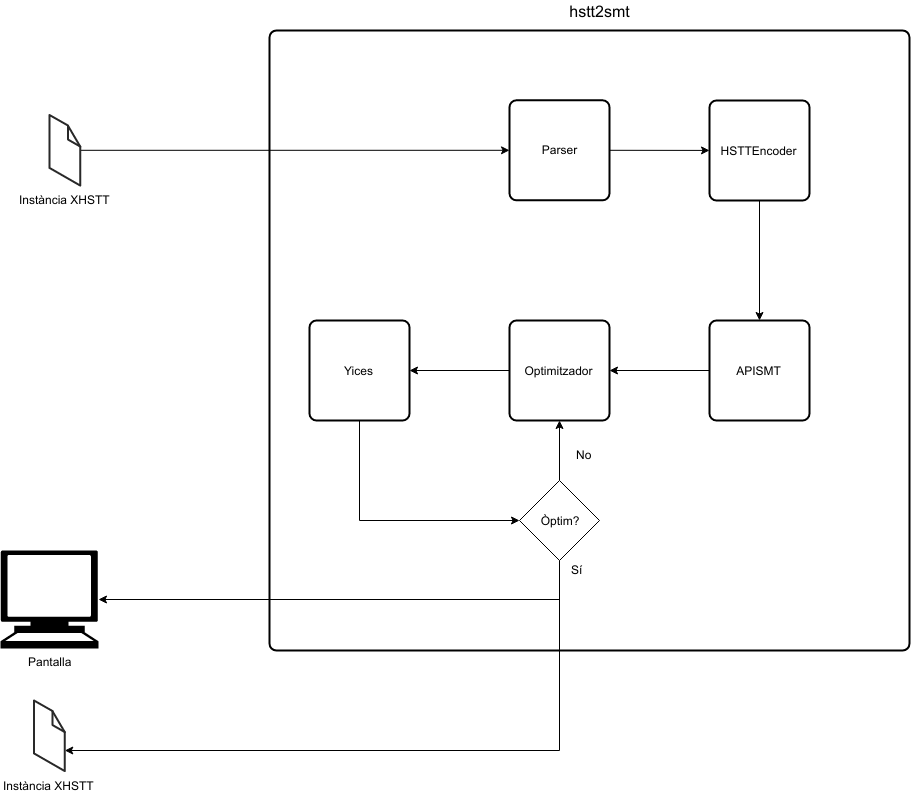
\includegraphics[width=\textwidth]{Diagrames/Arqui1.png}
  \caption{Arquitectura del programa}
  \label{fig:Arqui1}
\end{figure}
 

  \chapter{Estudis i decisions}
  \section{Programari utilitzat}
  En aquesta secció del treball es veurà tot el programari que s'ha utilitzat per la confecció d'aquest.
  \subsection{Yices 2}
  \begin{figure}[ht!]
    \centering
    
\includegraphics[width=0.4\textwidth]{Diagrames/logoYices.png}
    \caption{Logo Yices 2}
    \label{fig:yices}
  \end{figure}
  El Yices 2 és un \textit{SMT Solver} \textit{Open Source}\footnote{Repositori GitHub: \url{https://github.com/SRI-CSL/yices2}} sota llicència GPL que decideix la satisfactibilitat de fòrmules que contenen símbols de funcions no interpretades amb igualtat, aritmètica real i entera, BitVectors, tipus escalars i tuples. El Yices 2 suporta aritmètica linear i no linear.
  
  El Yices 2 pot processar fitxers d'entrada en notació SMT-LIB\footnote{\url{http://smtlib.cs.uiowa.edu/}}, es pot usar alternativament el llenguatge propi del Yices 2 i també te una API per C i C++.
  
  En la implementació d'aquest treball, s'usa dins de la API SMT del Dr. Jordi Coll com un dels \textit{solvers} que es poden utilitzar i és l'ùnic que permet SMT d'entre ells. S'ha decidit usar aquest a que és dels millors que hi ha i el grup de recerca hi te experiència prèvia. 

  S'ha utilitzat la versió 2.6.1.

  \subsection{pugixml}
  El pugixml és una llibreria C++ lleugera per al processament XML. És extremadament portable amb distribucions. També és opensource\footnote{Repositori GitHub: \url{https://github.com/zeux/pugixml}} sota llicència MIT.

  pugixml permet un processament de documents XML molt ràpid, còmode i eficient amb la memòria. Tot i això, al tenir un \textit{parser} DOM, no pot processar fitxers XML que no quèpiguen a la memòria.
  
  Degut a les caràcterístiques mencionades i a experiència prèvia amb la llibreria, s'ha decidit utilitzar-la per a la programació del \textit{parser} XHSTT. 

  S'ha utilitzat en la versió 1.9-1.

  \subsection{C++}
  \begin{figure}[ht!]
    \centering
    
\includegraphics[width=0.2\textwidth]{Diagrames/cpp.png}
    \caption{Logo C++}
    \label{fig:cpp}
  \end{figure}
  
  Llenguatge de programació de propòsit general creat per Bjarne Stroustrup com a extensió del llenguatge de programació C. 
  Des de llavors, el llenguatge s'ha expandit molt i el C++ permet programació orientada a objectes, genèrica i funcional, a més de facilitats per manipulació de memòria a baix nivell. 
  Pràcticament sempre és implementat com a llenguatge compilat.

  El compilador per a C++ que s'ha utilitzat es el G++ inclòs en el GNU Compiler Collection, que inclou compiladors per a C, C++, Objective-C, Fortran, Ada, Go i D, a més de llibreries per aquests llenguatges. 
  

  \begin{figure}[ht!]
    \centering
    
\includegraphics[width=0.2\textwidth]{Diagrames/gcc.png}
    \caption{Logo G++}
    \label{fig:gpp}
  \end{figure}


  En aquest treball s'ha decidit utilitzar el C++ perquè és amb el que es treballa al grup de recerca i és amb el que està feta la API SMT. El C++ s'ha utilitzat en la revisió C++17 del seu estandard. El GCC utilitzat ha estat en la versió 9.1.0-2. 

  \subsection{QtCreator}

  \begin{figure}[ht!]
    \centering
    
\includegraphics[width=0.2\textwidth]{Diagrames/qtc.png}
    \caption{Logo QtCreator}
    \label{fig:qtc}
  \end{figure}

  El QtCreator és un Entorn de Desoenvolupament Integrat (IDE de \textit{Integrated Development Environment}) multiplataforma per a C++, 
  JavaScript i QML que forma part del SDK per el \textit{framework} de desenvolupament d'aplicacions amb GUi Qt. Utilitza 

  S'ha utilitzat la versió 4.9.2-3.

  \subsection{\LaTeX}
  \begin{figure}[ht!]
    \centering
    
\includegraphics[width=0.4\textwidth]{Diagrames/latex.png}
    \caption{Logo \LaTeX}
    \label{fig:latex}
  \end{figure}
  

  Aquesta memòria s'ha confeccionat amb \LaTeX, que és un sistema de composició d'alta qualitat que inclou funcions dissenyades per a la creació de documents tècnics i científics amb la intenció de ajudar al creador a centrar-se més en el contingut que en la forma.
\LaTeX és l'estàndard de facto per a la comunicació i publicació de documents científics. 

Per la confecció i edició del document en sí, s'ha utilitzat l'editor Open Source\footnote{Link GitHub: \url{https://github.com/Microsoft/vscode}} Visual Studio Code. S'ha utilitzat en la versió 1.37.1-2 amb extensions per a facilitar l'edició del document tex.



  \subsection{GNU/Linux}
  \begin{figure}[ht!]
    \centering
    
\includegraphics[width=0.2\textwidth]{Diagrames/Linux.png}
    \caption{Logo Linux}
    \label{fig:linux}
  \end{figure}
  Linux és una familia de sistemes operatius formats pel \textit{kernel} Linux juntament amb les utilitats GNU. 
  El generador que s'ha fet en aquest treball ha estat desenvolupat per a linux, degut a la facilitat d'accés a les múltiples llibreries que s'han utilitzat, a que la API SMT ha estat desenvolupada també per a Linux i simplement per prèferencia personal, degut a que el sistema operatiu que utilitzo dia a dia és una distribució Linux.

  En concret s'ha treballat amb la distribució Arch Linux en la versió del kernel Linux 5.29.arch1-1 al final del treball (s'han usat versions anteriors que han anat sortint mentre es desenvolupava el treball).


  \section{Maquinari utilitzat}
  Per efectuar les proves de rendiment s'ha utilitzat un ordinador amb les següents especificacions:
  \begin{itemize}
    \item Processador AMD Ryzen\textsuperscript{TM} 3 1200 a 3.5 GHz amb 4 nuclis físics,  10MB de memòria cau i arquitectura 64 bits.
    \item 16GB de memòria RAM DDR4 a 3333MT.
    \item Sistema operatiu Arch Linux 64 bits amb kernel Linux 5.2.9.arch1-1
  \end{itemize} 
  


  \chapter{Anàlisis i disseny del sistema}

  \section{Anàlisis}
  % En la fase d’anàlisi cal detallar el model de dades i el model de processos. 
  \subsection{Necessitats del sistema}
  Les necessitats principals del sistema són les següents: 
  \begin{itemize}
    \item Necessitem rebre un fitxer de l'usuari.
    \item Necessitem llegir les dades de un fitxer XHSTT tal i com s'ha explicat anteriorment, per tant requerirem de un \textit{parser} per fer-ho.
    \item Necessitarem guardar les dades i les restriccions de alguna manera.
    \item Necessitarem un model lògic i codificar-lo utilitzant la API SMT del Dr. Jordi Coll. 
    \item Necessitarem processar i guardar les dades de manera que ens faciliti el mostrar-les de forma que es pugui entendre.
    \item Necessitarem comprovar en la mesura del possible que la instància XHSTT sigui correcta.
  \end{itemize}

  \subsection{Anàlisis de processos}
  L'usuari cridarà el programa, el programa llegirà el fitxer XHSTT que li ha passat l'usuari per paràmetre i s'encarregarà de codificar el model pel yices i cridar-lo per resoldre'l, utilitzant la llibreria per C++ pròpia del yices.
  %AMPLIAR + dibuixet un dibuixet amb lo de requeriments mes enfocat als processos


  
  \section{Disseny}    
  % En la fase de disseny cal determinar les interfícies d’usuaris, els models físics de 
  % dades, (no cal)els models físics de processos i, si escau, el model d’objectes. En aquest 
  % àmbit, els patrons de disseny permeten reutilitzar solucions generals a problemes 
  \subsection{Interfícies d'usuari}
  El programa funcionarà via consola. Les dades necessàries, com ara el fitxer amb la instància, es passaran per paràmetres, utilitzant el sistema existent en la API SMT del Dr. Jordi Coll.
  \subsection{Model de dades}

  El model de dades correspondria al següent diagrama:
  \begin{figure}[ht!]
    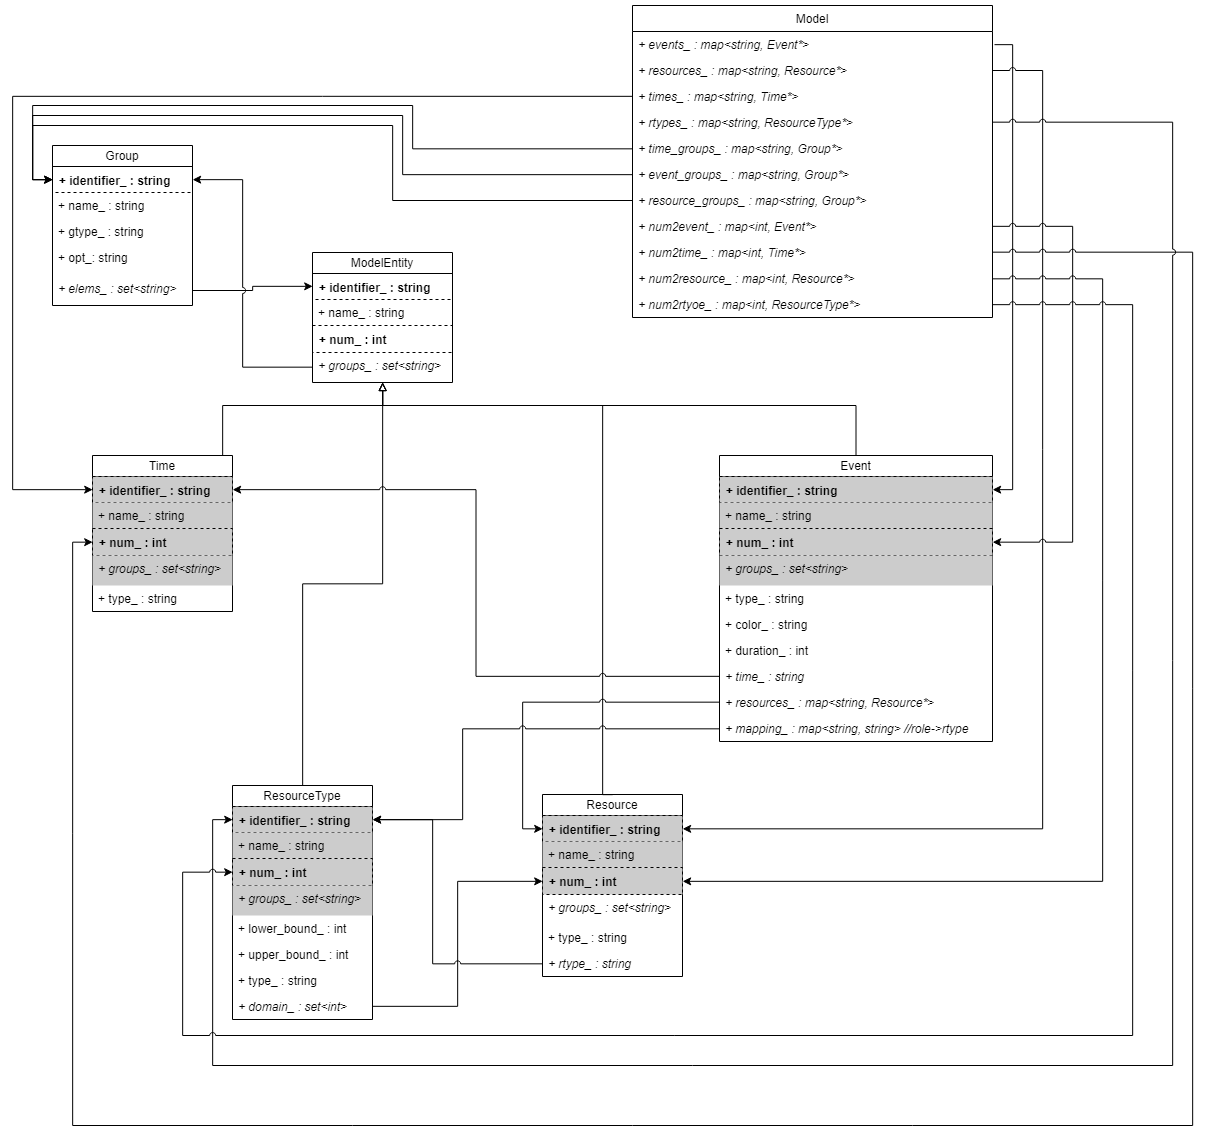
\includegraphics[width=\textwidth]{Diagrames/ModelDades.png}
    \caption{Model de Dades}
    \label{fig:DataModel}
  \end{figure}

  \subsection{Model d'objectes}

  El model d'objectes correspondria al següent diagrama:
  \begin{figure}[ht!]
    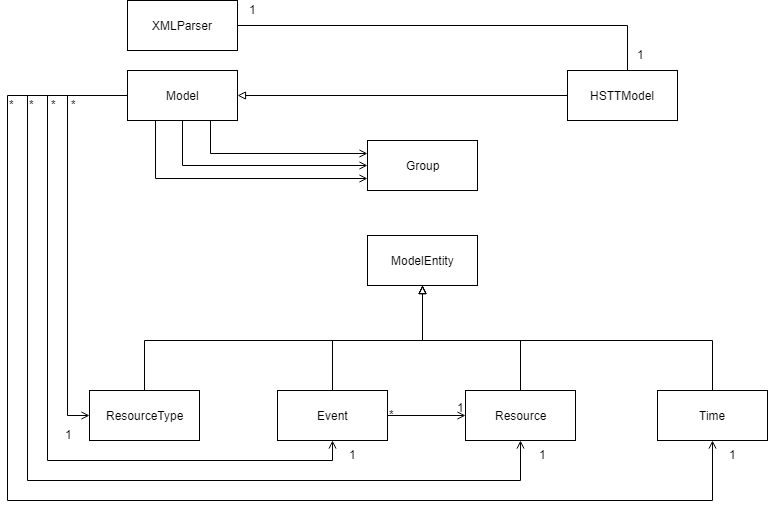
\includegraphics[width=\textwidth]{Diagrames/UMLKai.png}
    \caption{Model d'objectes}
    \label{fig:ObjectModel}
  \end{figure}
  



  

  \chapter{Implementació i proves}

  L'implementaci'o del generador s'he fet en C++, i està format per un conjunt de blocs definits:\
  \begin{itemize}
    \item \textit{Parser }del fitxer en format XHSTT. \\ S'encarrega de llegir el fitxer XHSTT i extreure'n la informació de la instància contenida en el fitxer XML en format XHSTT passat per parametre. És important que aquest fitxer tingui l'estructura establerta en el format XHSTT.
    \item Bloc de codificació de la instància a SMT. \\ En aquest apartat utilitzem la API SMT per tal de codificar la instància a SMT i passar-la al \textit{solver} corresponent, el Yices 2.
    \item Bloc de escriptura del resultat a XHSTT. \\ En aquest apartat creem un fitxer amb la instància treballada XHSTT i hi afegim la solució trobada al final.
  \end{itemize}

  L'usuari només tindrà un binari, anomenat \textit{hstt2smt}, amb el qual interectuarà per resoldre una instància que passarà per fitxer. Aquest s'encarregarà de fer tota la feina. 
  Aquest binari serà el resultat de compilar el generador amb la API SMT i les llibreries que es necessiten per poder treballar amb XML i amb SMT.
  %%%REVISAR%%%%%

  \section{Codificació}
  En aquesta secció es descriu la implementació de la codificació a SMT del generador d'horaris. 
  Posat que SMT no permet clausules violables, per a la codificació d'aquesta s'utilitzarà el cost i una variable auxiliar per cada clausula \textit{soft}, 
  que s'afegira a la seva corresponent clausula de forma condicional, negant la clausula inicial, de manera que si no es compleix la clausula inicial, la variable auxiliar hagi de ser certa. Al acabar la codifciació de la instància afegirem una clàusula pseudo-booleana amb totes les variables auxiliars amb els seus pesos, comparada amb un upperbound.
  Posat que la funció d'optimització serà la de minimitzar el cost total, el optimitzador anirà modificant el upperbound intentant reduir la funció objectiu, que també és el resultat exacte de la pseudo-booleana.

  Per exemple, si tenim les \textit{soft-clauses} següents: $SC_1$, $SC_2$, $SC_3$ amb costos respectivament: $W_1$, $W_2$, $W_3$. 
  Creariem les variables auxiliars $Aux_1$, $Aux_2$ i $Aux_3$. Amb això creariem les següents clausules:
  \begin{gather*}
    \neg SC_1 \rightarrow Aux_1 \\
    \neg SC_2 \rightarrow Aux_2 \\
    \neg SC_3 \rightarrow Aux_3
  \end{gather*}

  Hi aplicariem Algebra de Bool per convertir a CNF i convertiriem les clausules que són tipus $\neg A \rightarrow B$ a $\neg (\neg A) \vee B$ i d'aquí eliminariem la doble negació, quedant $A \vee B$:
  \begin{gather*}
    \neg SC_1 \vee Aux_1 \\
    \neg SC_2 \vee Aux_2 \\
    \neg SC_3 \vee Aux_3
  \end{gather*}vee
  Així doncs, afegint la clausula pseudobooleana amb les variables auxiliars i els pesos, ens quedarien les següents clausules:
  \begin{gather*}
      SC_1 \vee Aux_1 \\
      SC_2 \vee Aux_2 \\
      SC_3 \vee Aux_3 \\
      Aux_1*W_1 + Aux_2*W_2 + Aux_3*W_3 <= UPPERBOUND
  \end{gather*}


  Aquesta codificació està pensada per resoldre instàncies en què tots els recursos estàn assignats a algun event, com ara les instàncies de Brazil que són en les que ens hem enfocat al desenvolupar el generador. 
  Aquesta particularitat ens permet simplificar l'espai de cerca degut a la reducció de la combinatòria del problema, i permet una codificació més simple i directe de les restriccions de que es compon.

  \subsection{Model}

  El model està pensat per treballar a centrant-nos en els Events, els quals podriem definir com una reunió a la que es presenten diferents recursos i la nostre feina és la de decidir en quins espais de temps dels disponibles fiquem cada reunió d'aquestes.

  Les variables del model són les següents:
  \begin{itemize}
    \item $Xt_{0,0} ... Xt_{|Events|-1,|Times|-1}$\\Per cada event tenim tantes variables com espais de temps tingui l'instància. Cada una d'aquestes variables indica si un event en un espai de temps, s'està celebrant o no. 
    Doncs si per l'event $e$ i l'espai $t$, $Xt_{e,t}$ és certa, vol dir que en el temps $t$, $e$ s'està celebrant.
    \item $Xs_{0,0} ... Xs_{|Events|-1,|Times|-1}$\\Per cada event tenim tantes variables com espais de temps tingui l'instància. Cada una de aquestes variables indica si un event comença en l'espai de temps representat. Un event comença en un espai de temps si no es donava en l'espai de temps anterior i/o si l'espai de temps és la primera hora del dia.
    Doncs si per l'event $e$ i l'espai $t$, $Xt_{e,t}$ és certa, vol dir que en el temps $t$, $e$ comença i que cap més variable $Xs_{e,i}$ serà certa i que la variable $Xt_{e,t}$ serà certa.
    %A continuar
 
  \end{itemize}
   
  % En aquest apartat es detallen els problemes i les solucions apareguts en la 
  % implementació, així com, si és el cas, el model de classes i els algorismes més 
  % rellevants. 
  
  % A més, cal detallar les proves, tant unitàries com de sistema, que es realitzen. 
    
  \chapter{Implantació i resultats}
  % Aquest apartat ha de descriure amb detall el procés de desenvolupament que ha 
  % calgut dur a terme per implantar el sistema desenvolupat. L’apartat de resultats ha 
  % de mostrar clarament el grau d’assoliment dels objectius, mitjançant exemples del 
  % funcionament d’allò que s’ha fet. 
   
  % Es revisarà i valorarà que el sistema desenvolupat compleixi amb la legislació i 
  % normatives vigents, especialment en el que fa referència a la llei orgànica de 
  % protecció de dades de caràcter personal (LOPD) i a la llei de serveis de la societat 
  % de la informació i comerç electrònic (LSSICE). 
   
  % A més, ha de mostrar que l’aplicació resultant del projecte fa les tasques 

  \chapter{Conclusions}
  %%diagrama de gantt... semblant pero diferent del inicial
  \chapter{Treball futur}

  \nocite{*}
  \chapter{Bibliografía}
  \printbibliography[heading=none]
  \chapter{Manual d'usuari i insta\l.lació}
  
  
  \end{document}